\documentclass[border=10pt]{standalone}
\usepackage[svgnames]{xcolor}
\usepackage{amsmath}
\usepackage{pgfplots}
\pgfplotsset{compat=newest}
\usepackage[sfdefault]{FiraSans}
\usepackage{FiraMono}
\renewcommand*\familydefault{\sfdefault}
\begin{document}
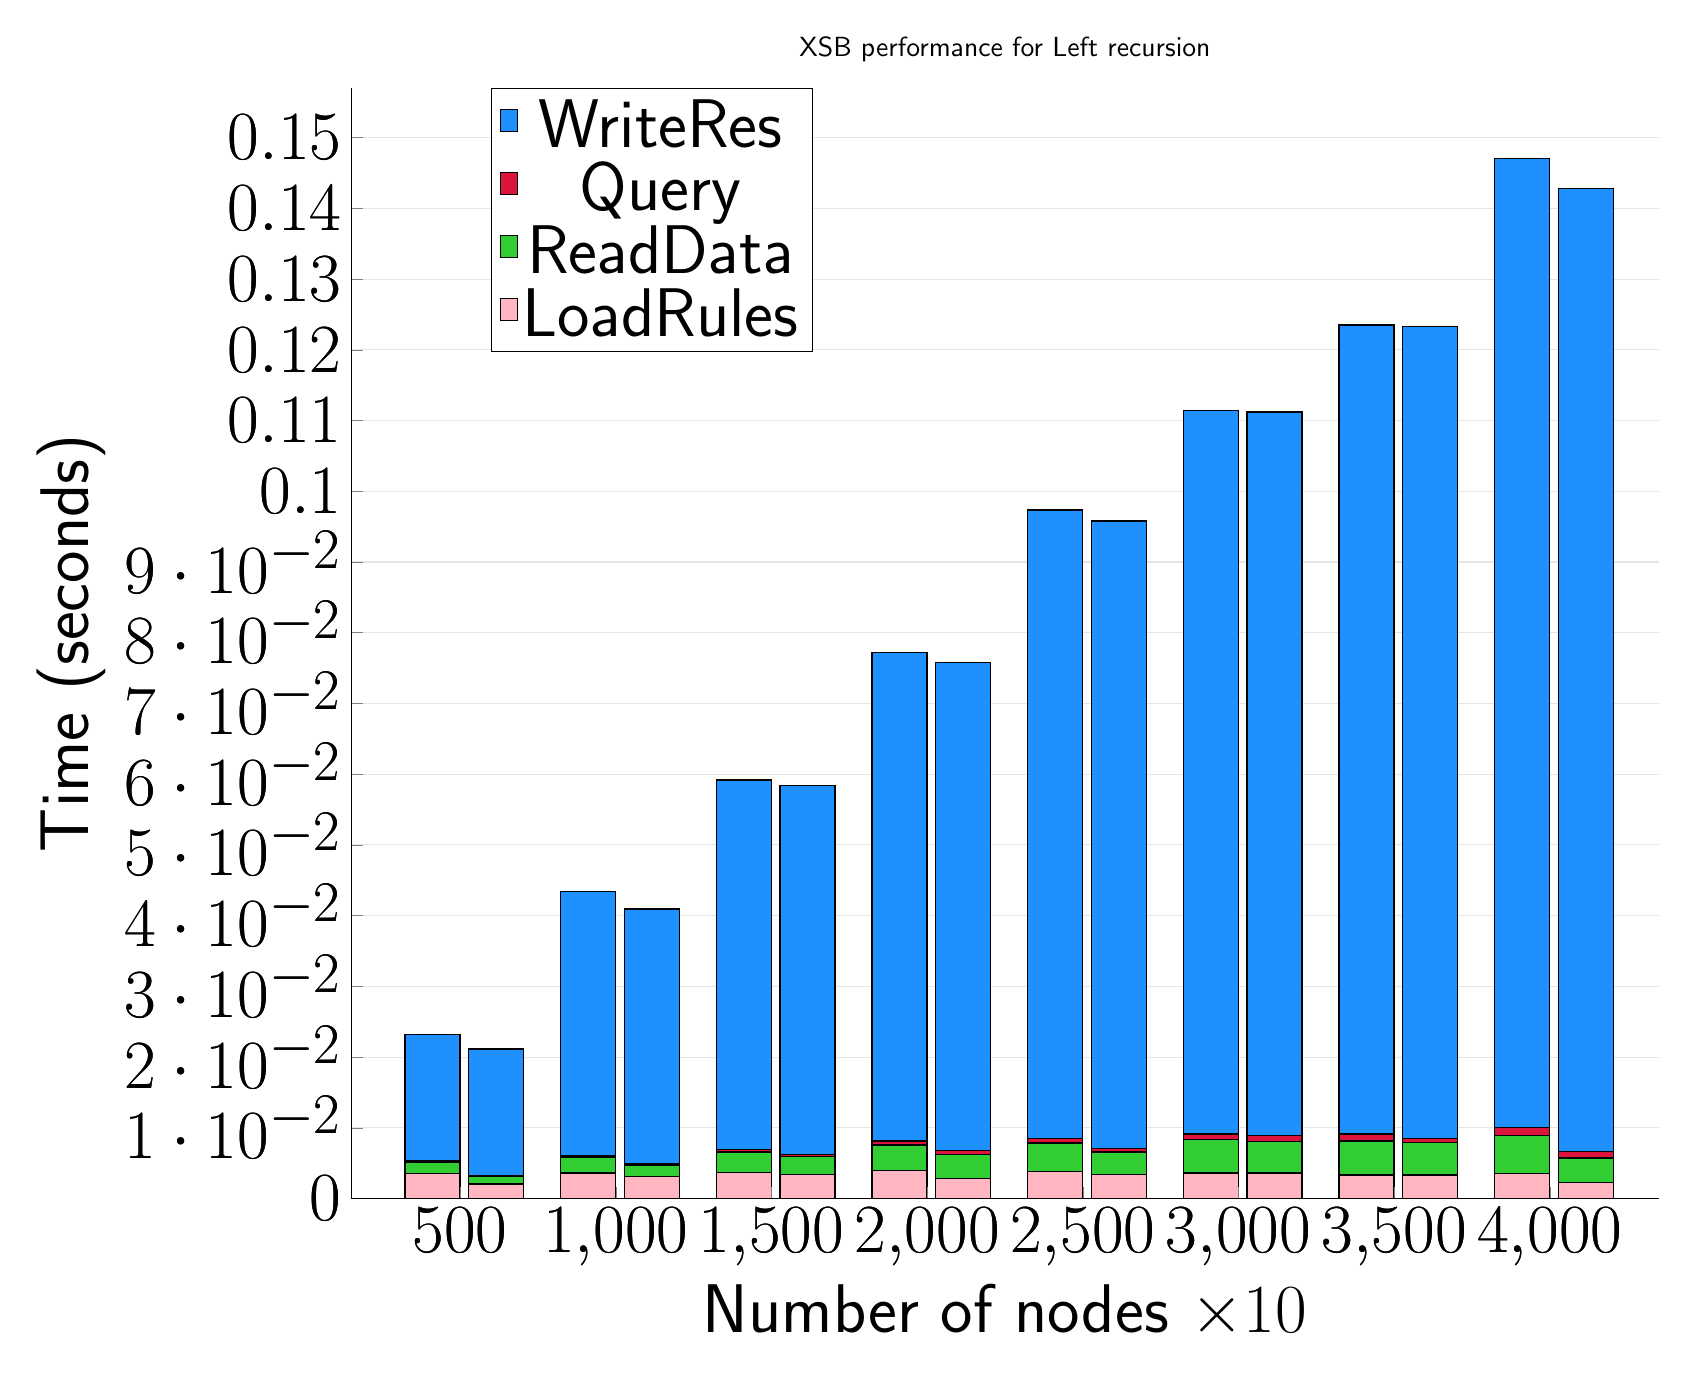
\begin{tikzpicture}
\begin{axis}[
   ybar stacked,
   title={XSB performance for Left recursion},
   bar shift=-10pt,
   width=1.5\textwidth,
   bar width=0.7cm,
   ymajorgrids, tick align=inside,
   major grid style={draw=gray!20},
   xtick=data,
   ymin=0, ymax=0.1570375951131183,
   axis x line*=bottom,
   axis y line*=left,
   enlarge x limits=0.1,
   legend style={
       at={(0.23, 1)},
       anchor=north,
       legend columns=1,
       font=\Huge,
   },
   ylabel={Time (seconds)},
   xlabel={Number of nodes $\times 10$},
   label style={font=\Huge},
   tick label style={font=\Huge},
]
\addlegendimage{fill=DodgerBlue, draw=black, line width=0.2pt}
\addlegendentry{WriteRes}
\addlegendimage{fill=Crimson, draw=black, line width=0.2pt}
\addlegendentry{Query}
\addlegendimage{fill=LimeGreen, draw=black, line width=0.2pt}
\addlegendentry{ReadData}
\addlegendimage{fill=LightPink, draw=black, line width=0.2pt}
\addlegendentry{LoadRules}
\addplot +[fill=LightPink, draw=black, line width=0.5pt] coordinates {
    (500, 0.003550608952840167)
    (1000, 0.0036409695943196633)
    (1500, 0.003698348999023436)
    (2000, 0.003972291946411134)
    (2500, 0.003812789916992187)
    (3000, 0.00362531344095866)
    (3500, 0.003357251485188803)
    (4000, 0.0035112698872884103)
};
\addplot +[fill=LimeGreen, draw=black, line width=0.5pt] coordinates {
    (500, 0.0016427040100097667)
    (1000, 0.002139568328857423)
    (1500, 0.002883354822794596)
    (2000, 0.0036067167917887364)
    (2500, 0.00404659907023112)
    (3000, 0.00468770662943522)
    (3500, 0.0048027833302815735)
    (4000, 0.0054473082224528)
};
\addplot +[fill=Crimson, draw=black, line width=0.5pt] coordinates {
    (500, 0.0001373291015625)
    (1000, 0.0002584457397460937)
    (1500, 0.000385284423828125)
    (2000, 0.0005843639373779297)
    (2500, 0.0005977948506673177)
    (3000, 0.0007916291554768881)
    (3500, 0.0009452501932779941)
    (4000, 0.0010627110799153667)
};
\addplot +[fill=DodgerBlue, draw=black, line width=0.5pt] coordinates {
    (500, 0.017877737681070968)
    (1000, 0.03737258911132814)
    (1500, 0.052224318186442076)
    (2000, 0.0690220991770426)
    (2500, 0.08890406290690105)
    (3000, 0.10231868426005042)
    (3500, 0.11442772547403968)
    (4000, 0.1370375951131183)
};
\end{axis}
\begin{axis}[
   ybar stacked,
   bar shift=13pt,
   width=1.5\textwidth,
   bar width=0.7cm,
   ymajorgrids, tick align=inside,
   major grid style={draw=none},
   xtick=data,
   ymin=0, ymax=0.1570375951131183,
   axis x line*=none,
   axis y line*=none,
   enlarge x limits=0.1,
   label style={font=\Huge},
   tick label style={font=\Huge},
]
\addplot +[fill=LightPink, draw=black, line width=0.5pt] coordinates {
    (500, 0.0020856666666666667)
    (1000, 0.00308)
    (1500, 0.003431333333333333)
    (2000, 0.0028513333333333338)
    (2500, 0.003385333333333329)
    (3000, 0.0036249999999999998)
    (3500, 0.0033399999999999997)
    (4000, 0.002300000000000003)
};
\addplot +[fill=LimeGreen, draw=black, line width=0.5pt] coordinates {
    (500, 0.0010366666666666666)
    (1000, 0.0016059999999999998)
    (1500, 0.0024813333333333332)
    (2000, 0.003335666666666667)
    (2500, 0.0031750000000000038)
    (3000, 0.004468666666666667)
    (3500, 0.004593333333333334)
    (4000, 0.0034366666666666664)
};
\addplot +[fill=Crimson, draw=black, line width=0.5pt] coordinates {
    (500, 9.300000000000168e-05)
    (1000, 0.0002159999999999997)
    (1500, 0.00035633333333333334)
    (2000, 0.0005833333333333313)
    (2500, 0.0005260000000000011)
    (3000, 0.0007916666666666674)
    (3500, 0.0005890000000000017)
    (4000, 0.0009456666666666672)
};
\addplot +[fill=DodgerBlue, draw=black, line width=0.5pt] coordinates {
    (500, 0.01792533333333333)
    (1000, 0.03604333333333334)
    (1500, 0.052163999999999995)
    (2000, 0.069014)
    (2500, 0.088723)
    (3000, 0.102327)
    (3500, 0.11474466666666666)
    (4000, 0.13611033333333333)
};
\end{axis}
\end{tikzpicture}

\end{document}
